\subsubsection{Frequência de Amostragem: 5 kHz}

Nesta seção, analisamos o comportamento de um sinal senoidal de 1 kHz com uma frequência de amostragem configurada para 5 kHz. Com essa taxa, coletamos um total de 200 amostras, permitindo observar o sinal no domínio do tempo e seu espectro de frequência.

\begin{figure}[H]
    \centering
    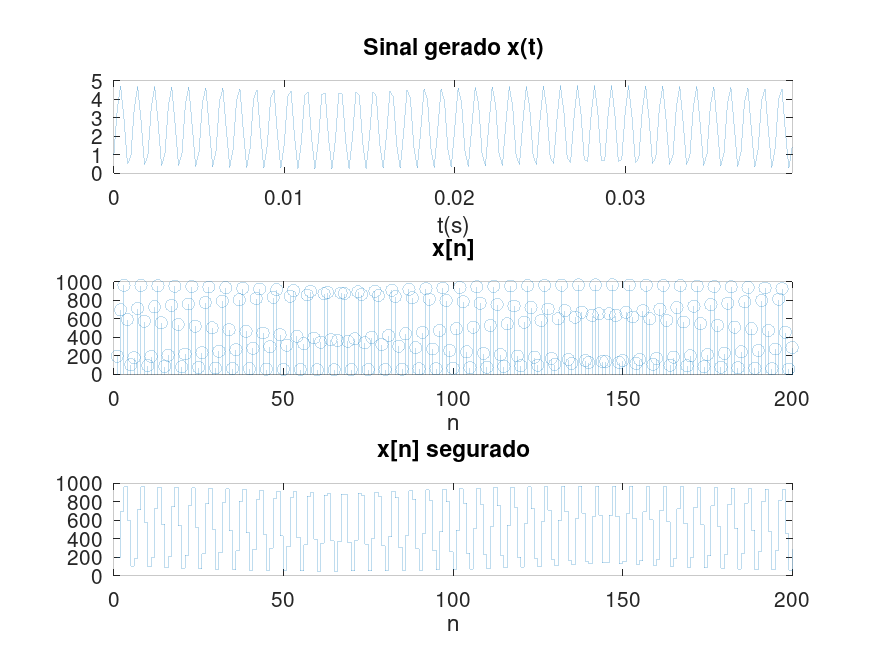
\includegraphics[width=1\linewidth]{03_results/assets/sin__1KHz_fs5k_SIGNAL_200smp.png}
    \caption{Sinal senoidal de 1 kHz com frequência de amostragem de 5 kHz, exibindo 200 amostras no domínio do tempo.}
    \label{fig:signal-5kHz-1kHz-200smp}
\end{figure}

\begin{figure}[H]
    \centering
    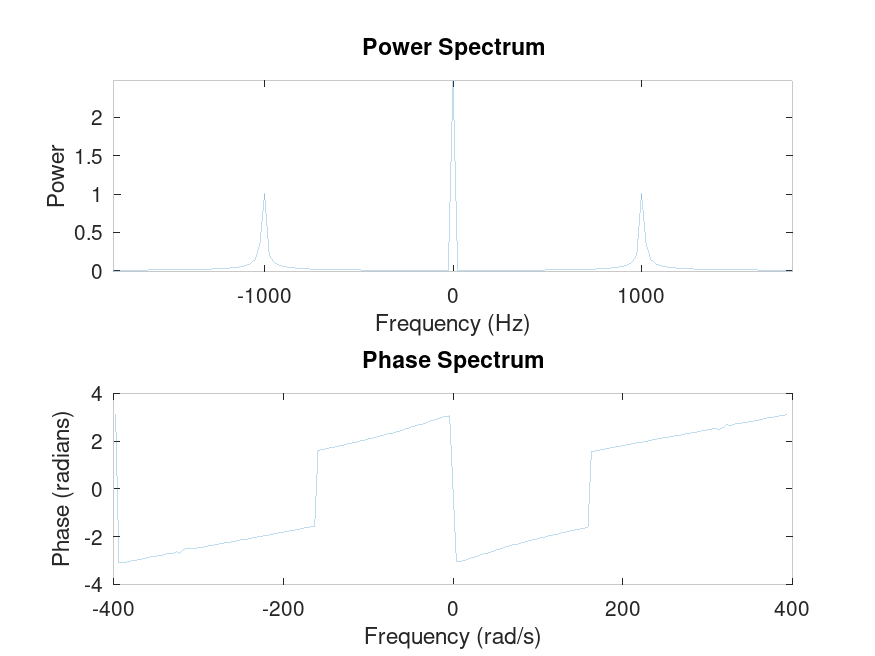
\includegraphics[width=1\linewidth]{03_results/assets/sin__1KHz_fs5k_SPECTRUM_200smp.png}
    \caption{Espectro do sinal senoidal de 1 kHz, amostrado a 5 kHz, com 200 amostras.}
    \label{fig:spectrum-5kHz-1kHz-200smp}
\end{figure}

\subsubsection{Frequência de Amostragem: 10 kHz}

Aqui, o sinal senoidal de 1 kHz foi amostrado a uma frequência de 10 kHz, permitindo uma coleta mais densa de pontos no domínio do tempo, totalizando 400 amostras.

\begin{figure}[H]
    \centering
    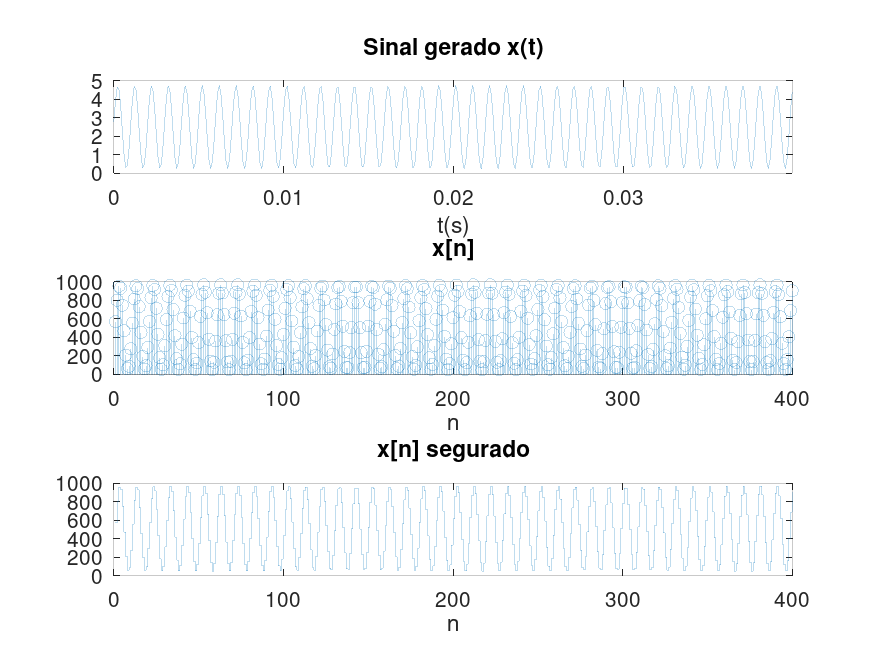
\includegraphics[width=1\linewidth]{03_results/assets/sin__1KHz_fs10k_SIGNAL_400smp.png}
    \caption{Sinal senoidal de 1 kHz amostrado a 10 kHz, apresentando 400 amostras no domínio do tempo.}
    \label{fig:signal-10kHz-1kHz-400smp}
\end{figure}

\begin{figure}[H]
    \centering
    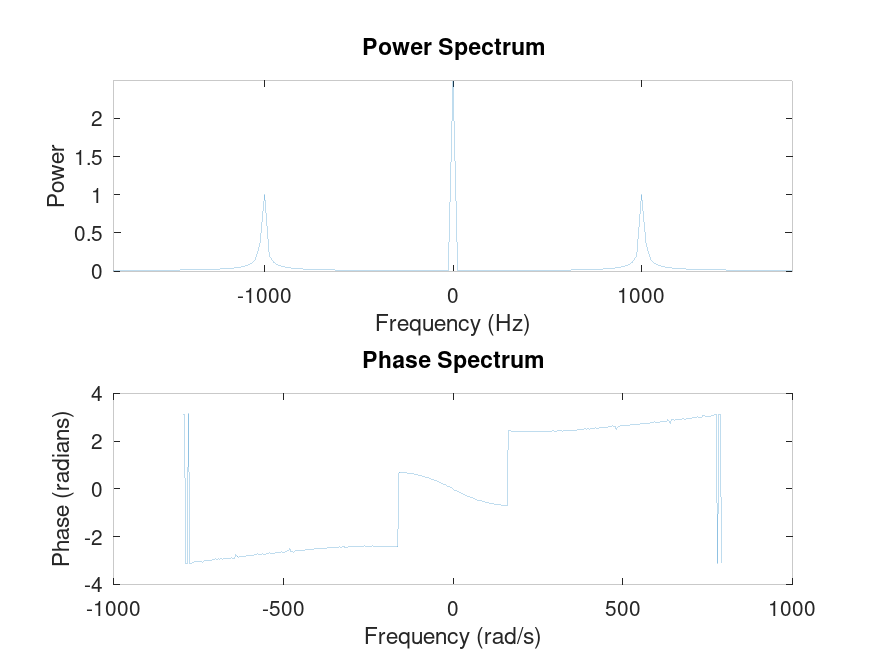
\includegraphics[width=1\linewidth]{03_results/assets/sin__1KHz_fs10k_SPECTRUM_400smp.png}
    \caption{Espectro do sinal senoidal de 1 kHz, com frequência de amostragem de 10 kHz e 400 amostras.}
    \label{fig:spectrum-10kHz-1kHz-400smp}
\end{figure}

\subsubsection{Frequência de Amostragem: 20 kHz}

Nesta seção, o sinal senoidal de 10 kHz foi amostrado a uma taxa de 20 kHz. Com essa configuração, coletamos 600 amostras, o que permite observar detalhadamente as características temporais e espectrais do sinal.

\begin{figure}[H]
    \centering
    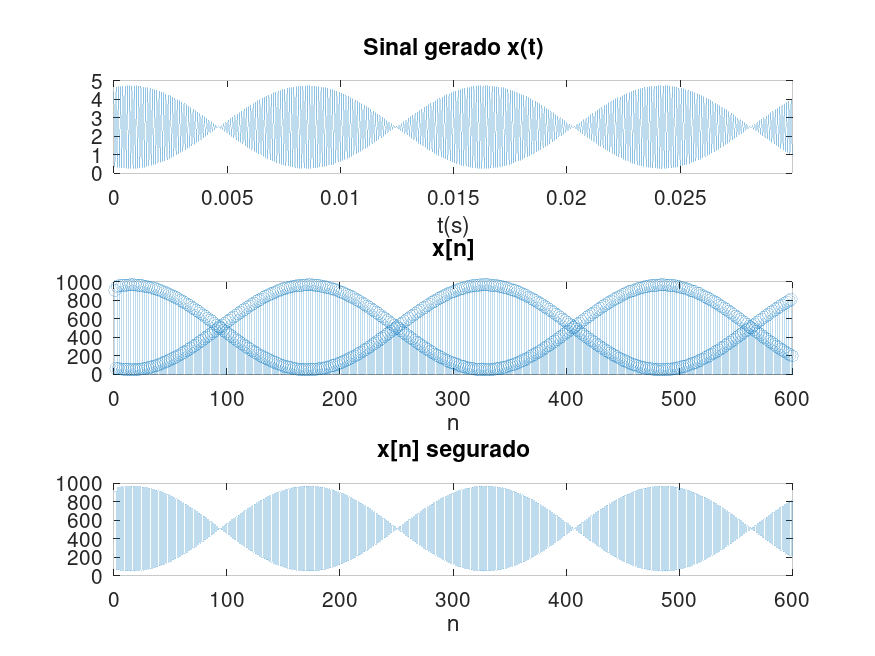
\includegraphics[width=1\linewidth]{03_results/assets/sin__10KHz_fs20k_SIGNAL_600smp.png}
    \caption{Sinal senoidal de 10 kHz com frequência de amostragem de 20 kHz, exibindo 600 amostras no domínio do tempo.}
    \label{fig:signal-20kHz-10kHz-600smp}
\end{figure}

\begin{figure}[H]
    \centering
    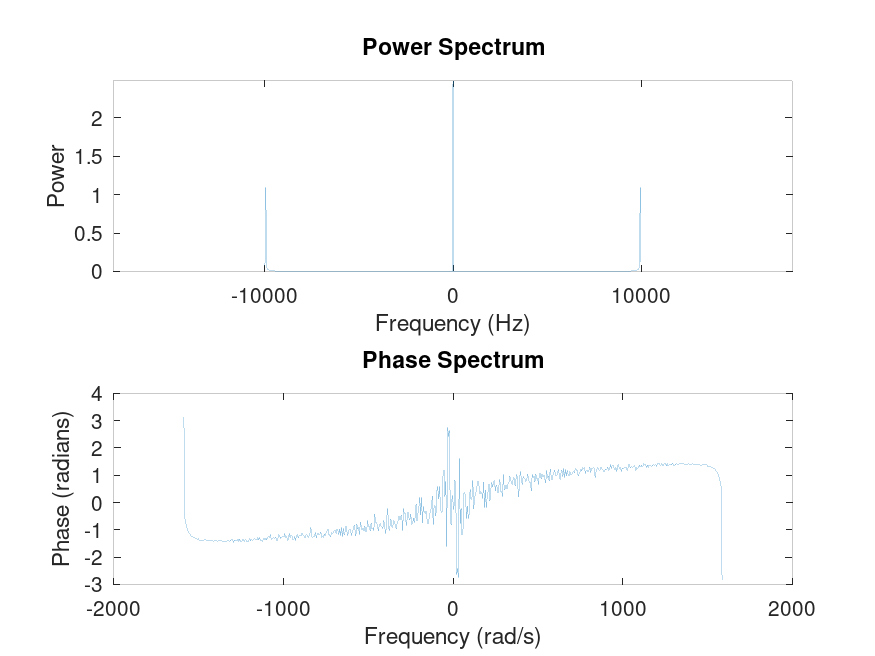
\includegraphics[width=1\linewidth]{03_results/assets/sin__10KHz_fs20k_SPECTRUM_600smp.png}
    \caption{Espectro do sinal senoidal de 10 kHz, amostrado a 20 kHz, com 600 amostras.}
    \label{fig:spectrum-20kHz-10kHz-600smp}
\end{figure}

\subsubsection{Frequência de Amostragem: 50 kHz}

Por fim, o sinal senoidal de 10 kHz foi amostrado a uma frequência de 50 kHz. Com essa configuração de alta resolução, obteve-se 600 amostras, permitindo uma análise detalhada no domínio do tempo e frequência.

\begin{figure}[H]
    \centering
    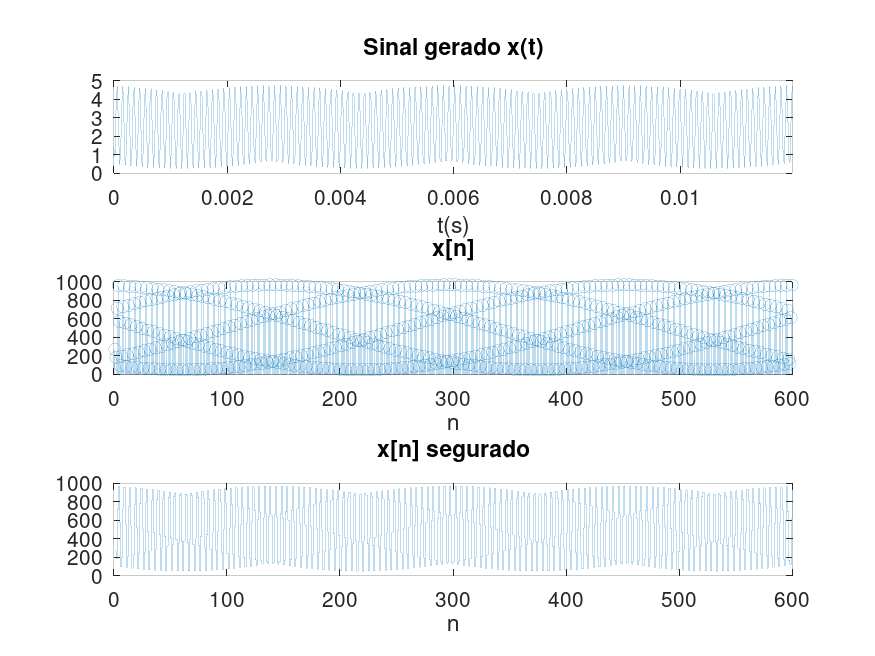
\includegraphics[width=1\linewidth]{03_results/assets/sin__10KHz_fs50k_SIGNAL_600smp.png}
    \caption{Sinal senoidal de 10 kHz com frequência de amostragem de 50 kHz, exibindo 600 amostras no domínio do tempo.}
    \label{fig:signal-50kHz-10kHz-600smp}
\end{figure}

\begin{figure}[H]
    \centering
    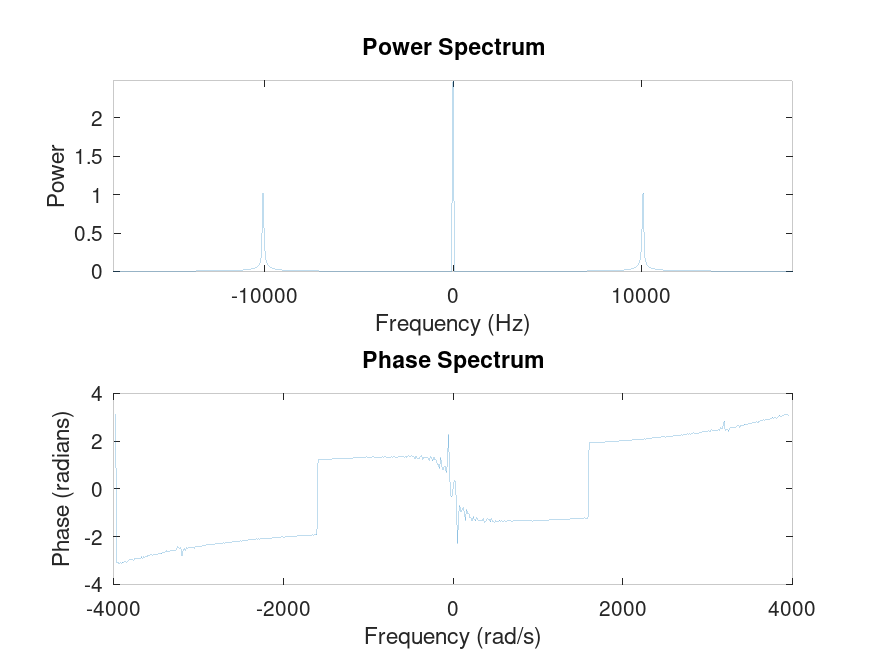
\includegraphics[width=1\linewidth]{03_results/assets/sin__10KHz_fs50k_SPECTRUM_600smp.png}
    \caption{Espectro do sinal senoidal de 10 kHz, amostrado a 50 kHz, com 600 amostras.}
    \label{fig:spectrum-50kHz-10kHz-600smp}
\end{figure}

\begin{itemize}
    \item Com o aumento da frequência de amostragem, o espectro do sinal representa com mais precisão a frequência original. Por exemplo, para um sinal de 1 kHz, uma amostragem de 5 kHz oferece resolução aceitável, mas com possíveis distorções no pico de frequência devido à menor densidade de amostras. Em frequências de amostragem mais altas, como 10 kHz ou 20 kHz, o espectro apresenta um pico mais claro e preciso, indicando menor quantização e menos aliasing.
    
    \item A quantidade de amostras também afeta a resolução espectral. Com 200 ou 400 pontos, o espectro apresenta picos mais largos e menos nítidos. Ao aumentar para 600 amostras, os picos de frequência ficam mais estreitos e definidos, pois o intervalo entre as frequências discretas diminui, proporcionando um espectro mais detalhado.
\end{itemize}
